\documentclass[]{article}

\usepackage[UTF8]{ctex}
\usepackage[graphicx]{realboxes}
\usepackage{caption} 
\usepackage{multirow}
\usepackage{amsmath}


\title{电子线路实验报告}
\author{陈祎睿\quad 电子信息\quad 2023302121299}

\begin{document}

\maketitle




\section{实验原理}

\subsection{二极管伏安特性实验}
二极管是一种只允许电流单向流动的半导体器件。

二极管具有单向导电性:二极管由P型和N型半导体材料构成,当正向偏置(P端接正,N端接负)时,二极管导通;反向偏置时,二极管截止。

在二极管导通的状态下,通过改变整体电路的电压,测量二极管的导通压降以及导通电流。二极管理论伏安特性曲线如下图。

\begin{figure}[htbp]
	\centering
	\captionsetup{font={small}}
	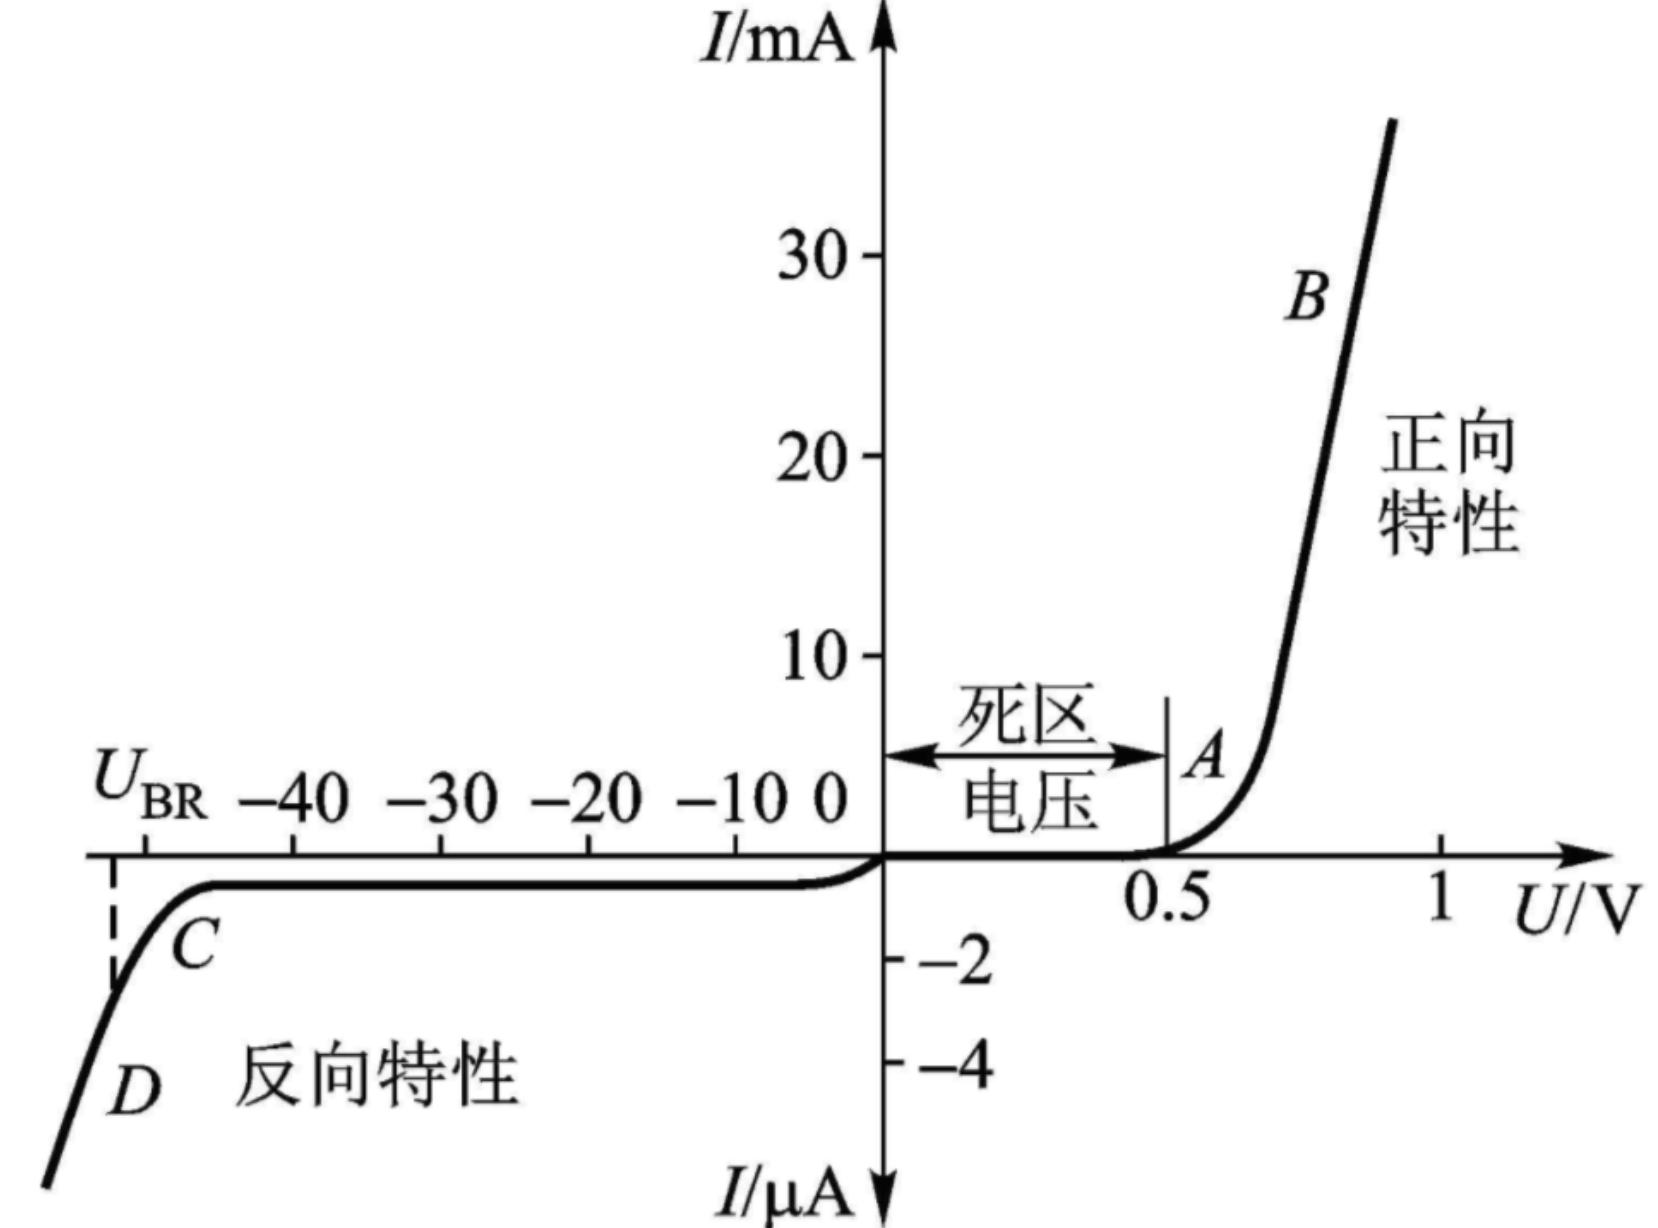
\includegraphics[height=3cm]{img/2_1}
	\caption{二极管理论伏安特性曲线图}
\end{figure}

\subsection{三极管放大电路的仿真与设计}

三极管,也称为晶体三极管或双极型晶体管,是一种用于放大或开关电子信号的半导体器件。它由三个主要部分组成:发射极、基极和集电极。三极管的工作原理基于半导体材料的能带结构和PN结的特性。

三极管共射放大电路是最基本的三极管放大电路之一,它以三极管的发射极为输出信号的公共端而得名。这种电路配置因其简单性和良好的高频特性而被广泛应用于各种电子设备中。

共射放大电路主要由以下部分组成:

\begin{enumerate}
	\item \textbf{三极管}:作为放大器的核心,可以是NPN型或PNP型。
	\item \textbf{偏置电路}:包括基极偏置电阻(Rb)和发射极偏置电阻(Re),用于设置三极管的工作点,确保三极管在放大区工作。
	\item \textbf{输入信号源}:连接在基极和地之间,提供需要放大的输入信号。
	\item \textbf{负载电阻}:连接在集电极和电源之间,作为放大电路的负载。
	\item \textbf{直流电源}:提供三极管工作所需的直流电压。
\end{enumerate}

该电路具有高输入阻抗、低输出阻抗、优良的放大效果、较好的频率响应的特点,因而广泛应用于各类电子设备当中。


\section{仪器设备}

\subsection{二极管伏安特性实验}
学生电源、二极管、万用表、电阻

\subsection{三极管放大电路的仿真与设计}
Tina-TI 电路仿真软件、三极管、万用表、10uF 电容、100uF 电容、不同阻值的电容,信号源、示波器、学生电源。

\begin{figure}[h]
	\centering
	
	\begin{minipage}{0.4\linewidth}
		\centering
		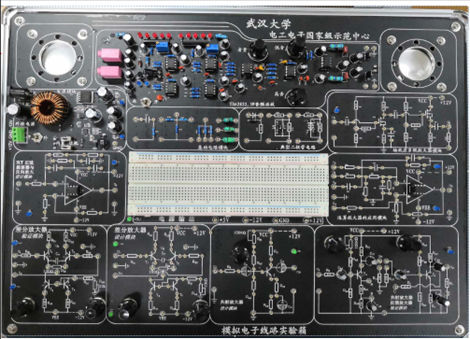
\includegraphics[width=4cm]{img/3_1}
	\end{minipage}
	\begin{minipage}{0.4\linewidth}
		\centering
		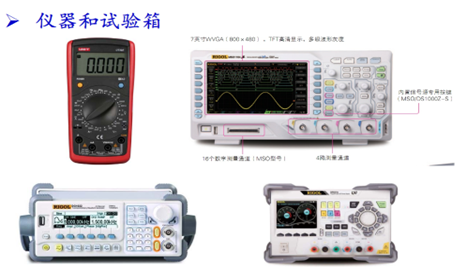
\includegraphics[width=5cm]{img/3_2}
	\end{minipage}
	
	\captionsetup{font={small}}
	\caption{仪器与试验箱}
	
\end{figure}


\section{实验步骤}

\subsection{二极管伏安特性实验}

使用串联电路来,保持电路中通过的电流处处相等,在电路中串联一个保护电阻,以防止电路中的电流过大,最终导致二极管损坏。测量电流值时,将万用表调至电压挡串联在电路中。测量电压时,将万用表调至电流挡并联在二极管的两端。仿真电路图如图3。



\subsection{三极管放大电路的仿真与设计}

按照三极管共射极放大电路的基本原理,设计实验电路。首先,在仿真软件绘制实验电路图,比对电路指标,验证电路的可行性。仿真电路图如图4。


\begin{figure}[h]
	\centering
	
	\begin{minipage}{0.4\linewidth}
		\centering
		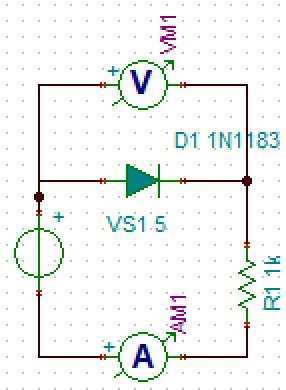
\includegraphics[width=2cm]{img/4_1}
		\captionsetup{font={small}}
		\caption{二极管伏安特性实验仿真电路图}
	\end{minipage}
	\begin{minipage}{0.4\linewidth}
		\centering
		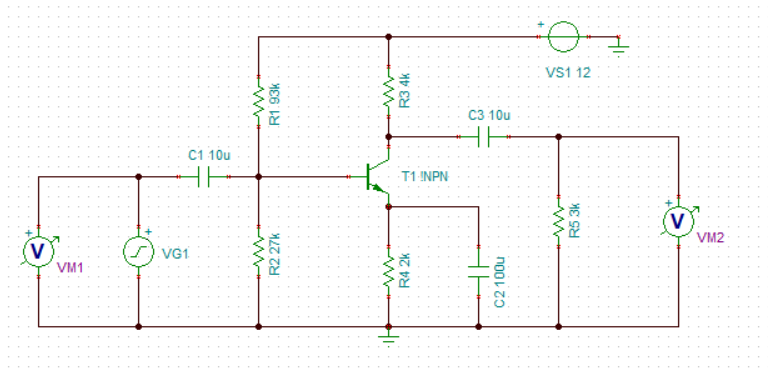
\includegraphics[width=5cm]{img/4_2}
		\captionsetup{font={small}}
		\caption{三极管共射级放大电路仿真电路图}
	\end{minipage}

\end{figure}


仿真得到实验的静态工作点和动态放大特性,设定直流输入为12V,交流输入为5mv,频率1000Hz。仿真结果如图5。

使用光标测量两波形的顶点,得到A1=-55


\begin{figure}[h]
	\centering
	
	\begin{minipage}{0.4\linewidth}
		\centering
		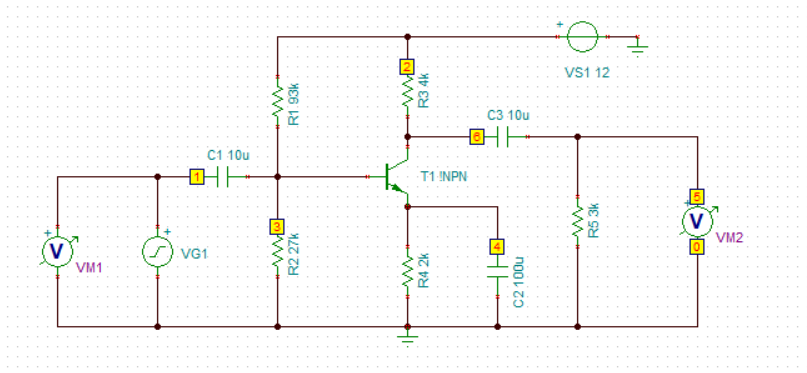
\includegraphics[height=2.5cm]{img/4_3}
		\captionsetup{font={small}}
		\caption{直流结果分析节点示意图}
	\end{minipage}
	\begin{minipage}{0.4\linewidth}
		\centering
		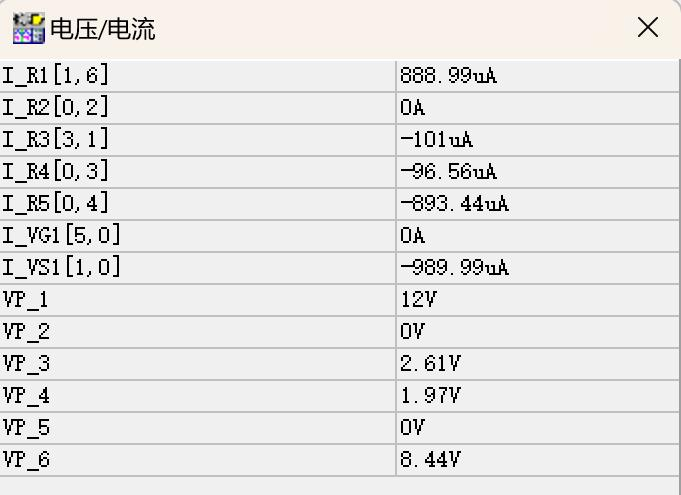
\includegraphics[height=2.5cm]{img/4_4}
		\captionsetup{font={small}}
		\caption{直流通路仿真结果表}
	\end{minipage}
	
\end{figure}

\begin{figure}[h]
	\centering
	
	\begin{minipage}{0.4\linewidth}
		\centering
		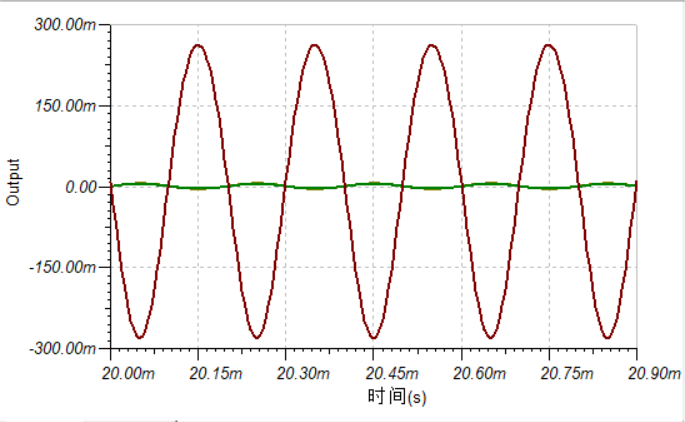
\includegraphics[height=2.5cm]{img/4_5}
		\captionsetup{font={small}}
		\caption{交流通路输入输出仿真波形图}
	\end{minipage}
	\begin{minipage}{0.4\linewidth}
		\centering
		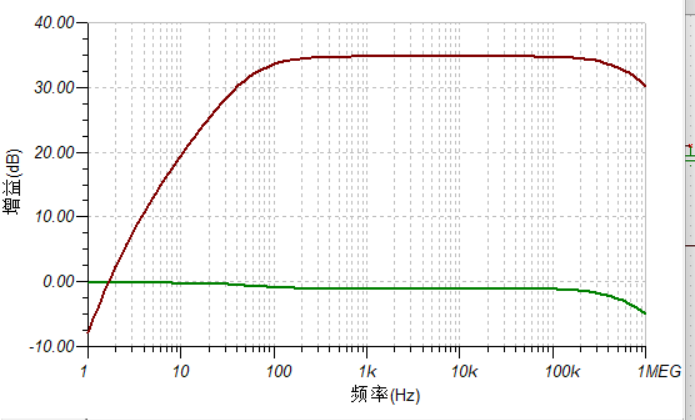
\includegraphics[height=2.5cm]{img/4_6}
		\captionsetup{font={small}}
		\caption{交流通路频率增益曲线图}
	\end{minipage}
	
\end{figure}

由于实验室条件限制,没有27000Ω、93000Ω和4000Ω的电阻,所以在尽可能不影响电路性能的情况下,更换电阻进行实验。将27000Ω电阻更换为30000Ω电阻,将93000Ω电阻更换为100000Ω电阻,将4000Ω电阻更换为3900Ω电阻,进行电路拼装与实验。



	将静态工作点做戴维南转化,其中$V_s = V_{cc} \cdot \frac{R_1}{R_1 + R_2} = 2.7V$, $R' = \frac{R_1 \parallel R_2}{R_1 + R_2} = \frac{R_1 \cdot R_2}{R_1 + R_2} = 20.925\Omega$。所以有 
	\[ V_s = I_{BQ} \cdot R' + 0.7 + (\beta + 1) I_{BQ}, \]
	解得,$I_{BQ} = 0.003mA$, $I_{CBQ} = \beta I_{BQ} = 0.965mA$, 所以,$I_{BQ}$ 仿真与工程计算之间的误差 $\delta = \left( \frac{0.003 - 0.00293349}{0.003} \right) \times 100\% = 2.2\%$,可见,仿真分析在一定程度上与工程近似计算相一致。
	
	由此可知,电压增益 $A_v = \frac{U_2}{U_1} = \frac{384.267}{6.463} = 59.46$,也可由示波器上的波形图粗略计算 $A_v = \frac{V_{ppb}}{V_{ppa}} = \frac{493.000}{8.963} = 55.00$。由于手动滑动光标,很难让其停在峰值位置,所以用仿真的波形图测出的电压增益没有用万用表测出的增益准确。所以仿真的电压增益我们取 $A_v = 59.46$。
	
	\[ r_{be} = 200 + \frac{(\beta + 1) V_T}{I_{EQ}} = 8867\Omega, \]
	\[ V_i = i_b \cdot r_{be}, \quad V_o = -\beta i_b \left( \frac{R_c \parallel R_L}{R_c + R_L} \right), \]
	故求得 
	\[ A_v = \frac{V_o}{V_i} = -\frac{\beta \left( \frac{R_c \parallel R_L}{R_c + R_L} \right)}{r_{be}} = -69.3. \]
	可见,工程计算与仿真分析的增益误差 $\delta = \left( \frac{61.29 - 59.46}{69.3} \right) \times 100\% = 2.99\%$,比较接近。
	


\section{实验数据}

\subsection{二极管伏安特性实验}


\begin{table}[htbp]
	\centering
	\captionsetup{font={small}}
	\caption{二极管伏安特性实验数据记录表}
	
	\begin{tabular}{llllllll}
		\hline
		$ V_{DD} $ & 0.37     & 0.52    & 0.635 & 0.648 & 0.672 & 0.693 & 0.709 \\
		\hline
		$ I_D $  & 0.000012 & 0.00031 & 0.001 & 0.002 & 0.003 & 0.004 & 0.005 \\
		\hline
		\hline
		$ V_{DD} $ & 0.723     & 0.734    & 0.745 & 0.756 & 0.778 & 0.786 & 0.801 \\
		\hline
		$ I_D $  & 0.006 & 0.007 & 0.008 & 0.009 & 0.010 & 0.011 & 0.012 \\
		\hline
		\hline
		$ V_{DD} $ & 0.822     & 0.839    & 0.847 & 0.863 & 0.872 & 0.687 & 0.911 \\
		\hline
		$ I_D $  & 0.013 & 0.014 & 0.015 & 0.016 & 0.017 & 0.018 & 0.019 \\
		\hline
	\end{tabular}
	
\end{table}


\subsection{三极管放大电路的仿真与设计}

\subsubsection{静态测量}
见表2
\begin{table}[h]
	\centering
	\captionsetup{font={small}}
	\caption{三极管放大电路静态测量数据记录表}
	
	\begin{tabular}{llllll}
		\hline
		 $ V_{CQ} $  & $ V_{EQ} $    & $ V_{BQ} $   & $ V_{CEQ} $ & $ V_{BEQ} $ & $ I_{CQ} $  \\
		\hline
		 12.12V & 2.34V & 2.7V & 9.28V & 0.621V & 1.23mA \\
		\hline
		
	\end{tabular}
	
\end{table}


\subsubsection{动态测量}
见表3、4、5、6(在第7页),图9

\begin{table}[h]
	\centering
	\captionsetup{font={small}}
	\caption{三极管放大电路电压增益数据记录表}
	
	\begin{tabular}{lll}
		\hline
		测试项目  & 名目    & 测试值  \\
		\hline
		\multirow{2}*{输入} & f(Hz) & 1000 \\
		\cline{2-3}
		~ & Vi(mV) & 4.4 \\
		\hline
		\multirow{2}*{输出} & Vi(mV) & 297.5 \\
		\cline{2-3}
		~ & Av & -69.3 \\
		\hline
	\end{tabular}
	
\end{table}

\begin{figure}[htbp]
	\centering
	\captionsetup{font={small}}
	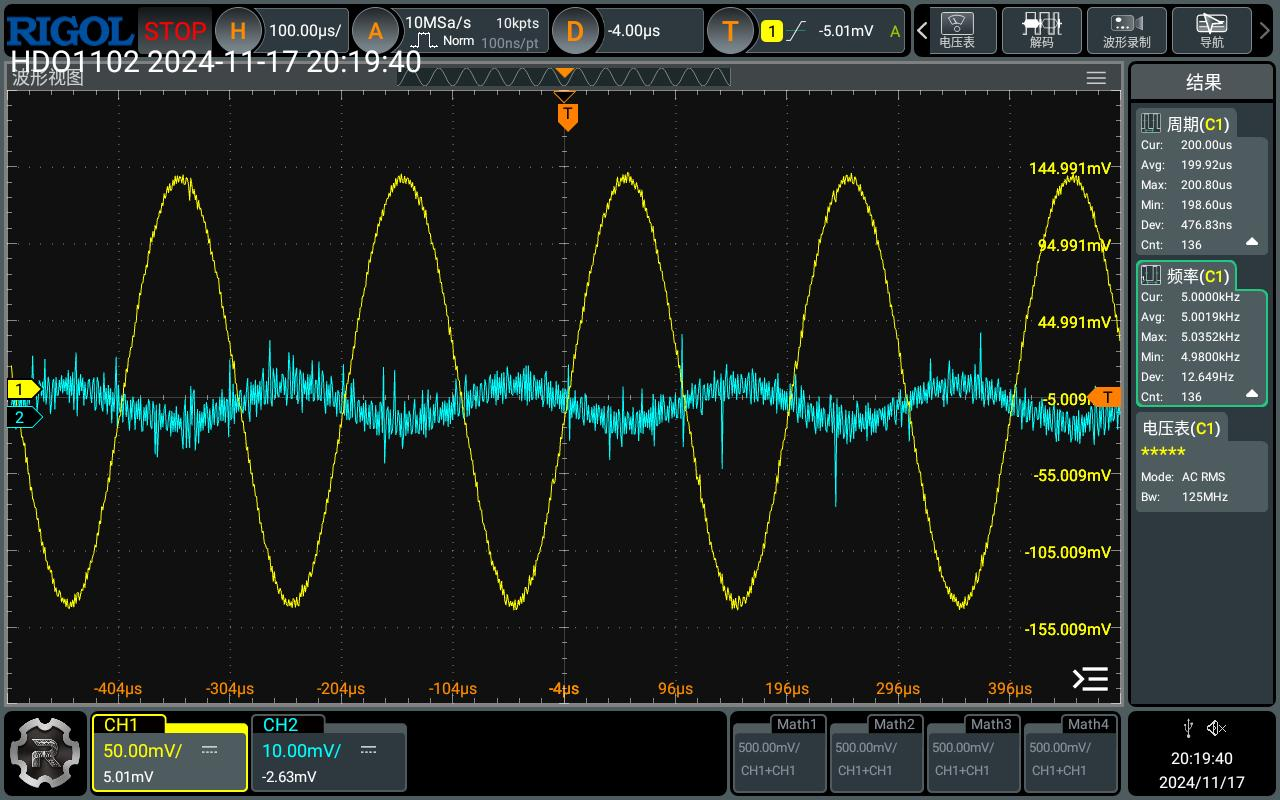
\includegraphics[height=4cm]{img/5_1}
	\caption{示波器输出波形图}
\end{figure}

\begin{table}

	\centering
		
	\begin{minipage}{0.9\linewidth}
		\centering
		\captionsetup{font={small}}
		\caption{三极管放大电路输入电阻数据记录表}
		
		\begin{tabular}{lll}
			\hline
			项目  & 测试值    & 说明  \\
			\hline
			Vi(mV) & 4.4 & 输入端信号幅度 \\
			\hline
			Vs(mV) & 5 & 信号源信号幅度 \\
			\hline
			Rs($ \Omega $) & 500 & 内阻 \\
			\hline
			Ri($ \Omega $) & 3628.1 & 计算输入电阻 \\
			\hline
		\end{tabular}
	\end{minipage}
	
	\begin{minipage}{0.9\linewidth}
		\centering
		\captionsetup{font={small}}
		\caption{三极管放大电路输出电阻数据记录表}
		
		\begin{tabular}{lll}
			\hline
			项目  & 测试值    & 说明  \\
			\hline
			Vo(mV) & 291.4 & 负载开路输出大小 \\
			\hline
			$ V_{OL} $(mV) & 135.2 & 带负载输出大小 \\
			\hline
			$ R_L $ ($ \Omega $) & 300 & 测量负载电路 \\
			\hline
			Ro($ \Omega $) & 3589.3 & 计算输出电阻 \\
			\hline
		\end{tabular}

	\end{minipage}

\end{table}




\begin{table}[h]
	\centering
	\captionsetup{font={small}}
	\caption{二极管测试通频带数据记录表}
	
	\begin{tabular}{llllllllll}
		\hline
		f(kHz) & 0.05     & 0.1    & 0.2 & ... & 1.0 & ... & 30 & 50 & 81.2 \\
		\hline
		Vo  & 435 & 531 & 595 & ... & 635 & ... & 535 & 498 & 435 \\
		\hline
		Av  & 43.2 & 57.6 & 60.2 & ... & 69.3 & ... & 61.3 & 45.1 & 43.2 \\
		\hline
	\end{tabular}
	
\end{table}


\section{实验数据分析}

\subsection{二极管伏安特性实验}

绘制二极管伏安特性曲线。曲线图如图10。

\begin{figure}[h]
	\centering
	\captionsetup{font={small}}
	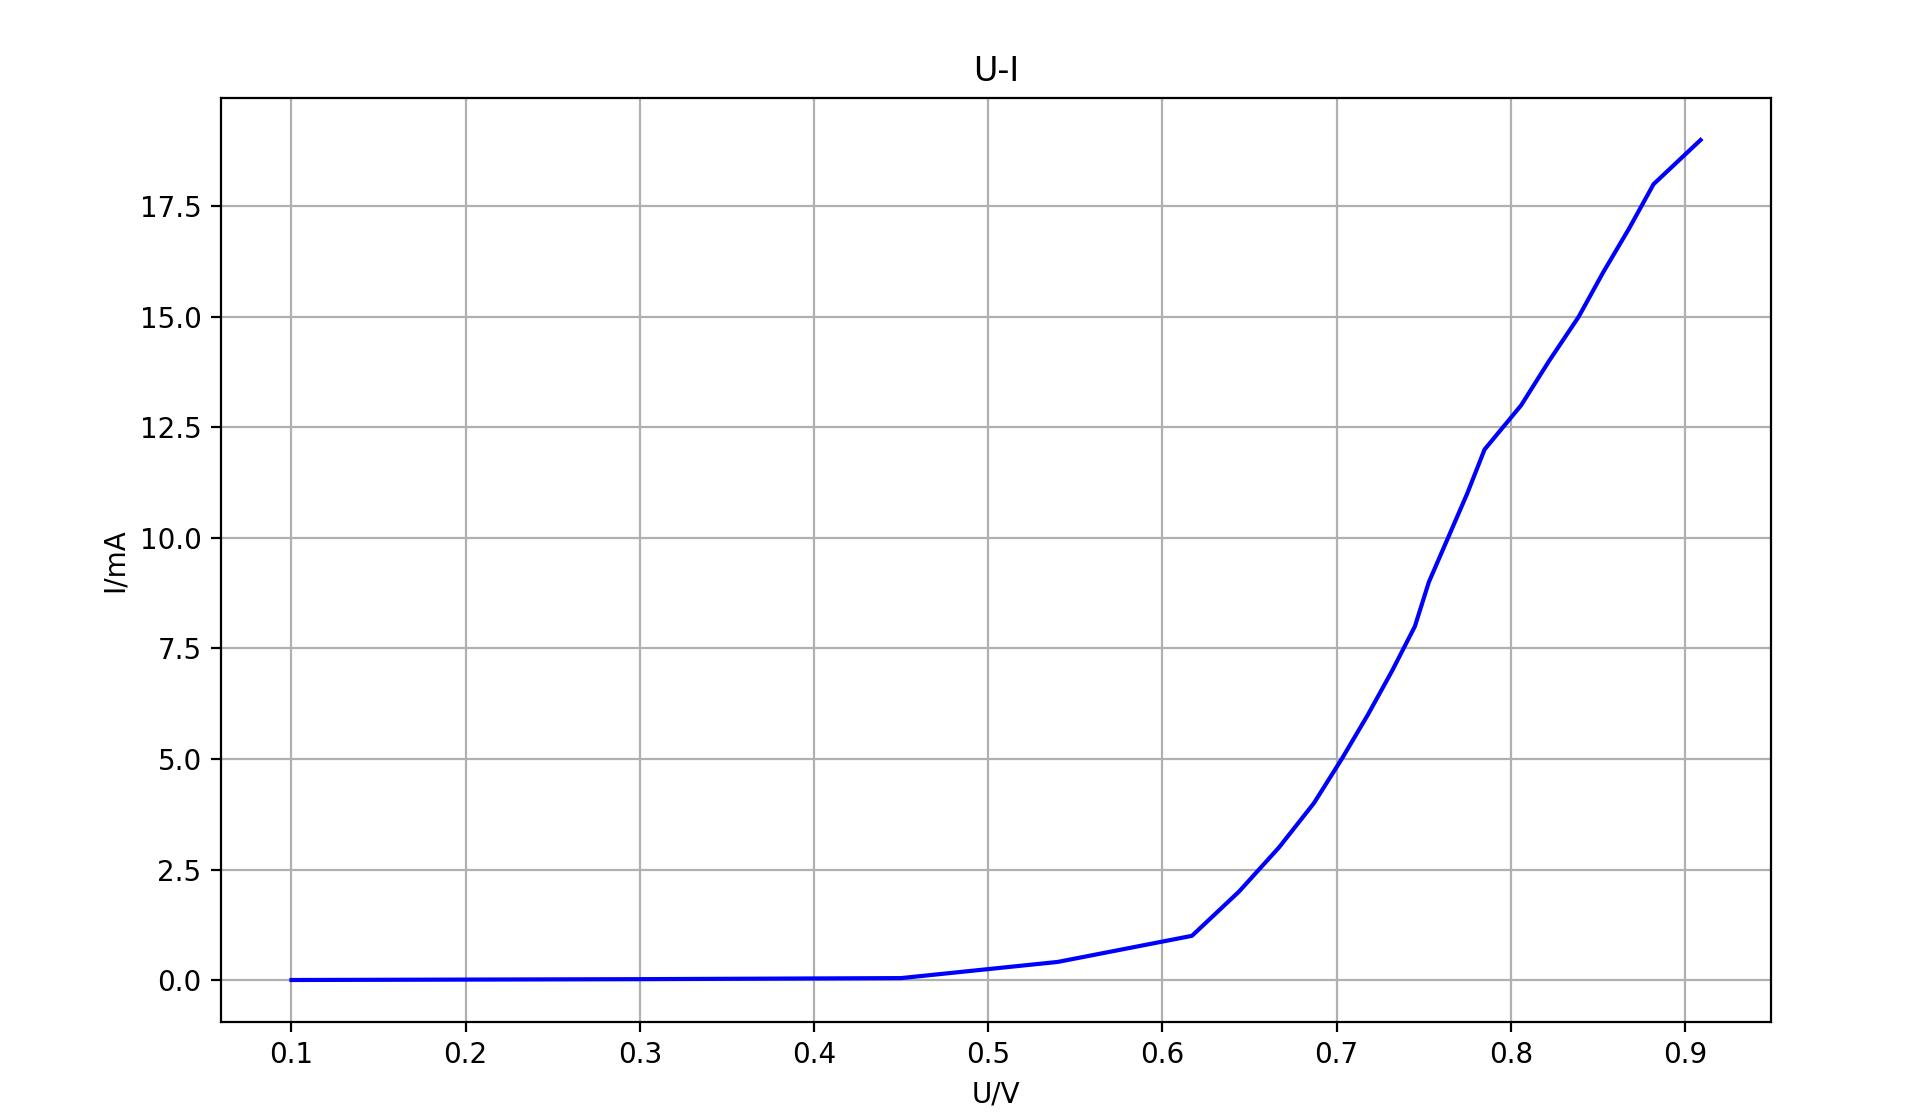
\includegraphics[height=4cm]{img/6_1}
	\caption{二极管伏安特性曲线图}
\end{figure}

\subsection{三极管放大电路的仿真与设计}

实验测试的得到的静态工作点数据与模拟得到的理论数据接近,输出电压波动较小,放大效果明显,放大倍数为69.3,与实验要求的50接近,实验基本成功。

\section{实验思考与分析}

\subsection{在负载确定且输出阻抗不宜太大时,提高电压增益有什么方法?}

可以提高电源电压或者减小$R_{b1}$和$R_{b2}$,$R_e$的值。由
\[ A_s = -\beta \left( \frac{R_c // R_L}{r_{be}} \right), \]
当$R_c$和$R_L$确定时,可以减小$r_{be}$的值,增大静态工作时$I_{BQ}$的值。提高电源电压$V_{cc}$或者减小$R_{b1}$和$R_{b2}$可以提高$I_{BQ}$的值。



\subsection{增大Rc可有效提升电压增益,但容易引起什么失真?}

容易引起饱和失真。Rc 增大会引起集电极电压下降,此时Rc 与Vcc 的伏安曲线整
体向右偏,静态工作点右移,容易引起饱和失真。

\subsection{设计电路输入信号的最大振幅大约为多少?(提示:不引起失真)}

电路输入信号最大振幅 $V_m$ 为
\[ V_m = \min\{ V_{CEQ} - V_{CES}, I_{CQ} \cdot R_c' \}, \]
取 $V_{CES} = 0.6V$,$V_{CEQ} - V_{CES} = 8.63V$,$I_{CQ} \cdot R_c' = 1.368V$。所以,最大振幅约为 $1.368V$。

\subsection{调整输入信号的振幅(1mv~10mv),观察输出信号正、负振幅的差异,以及差异的变化趋势,思考差异产生的原因。}

负振幅绝对值小于正振幅绝对值,随着信号振幅的增大这种趋势越来越明显,原
因是随着信号的增大,开始出现饱和失真,信号越大,负振幅逐渐被$ V_{CES} $截断,正负振
幅差距不断增大。


\end{document}
